\chapter{基于粒子群算法的硬件加速补偿系统设计}
\section{硬件设计方法}
\subsection{流水线技术}
\label{流水线技术}
当前一般用吞吐率(throughput)作为硬件的性能指标,对于将要设计的用于干涉仪环境补偿的粒子群加速补偿模块,其吞吐率的计算公式可以使用下式:
\begin{equation}\label{eq:吞吐率计算}
    throughput = \frac{Operation}{second}=\frac{PSO}{instructions}\times \frac{instructions}{clock cycle} \times \frac{clock cycle}{time(1s)}.
    \end{equation}

式\eqref{eq:吞吐率计算}的含义为每秒钟能执行的操作数量,它由三部分组成:有效操作(PSO计算)占所有指令的比例$\frac{PSO}{instructions}$、每个周期能执行的指令数量$\frac{instructions}{clock cycle}$以及1秒钟内包含的周期个数$\frac{instructions}{clock cycle}$,其中前两项为强相关,可以合并为一个因素进行考虑,即一个周期能执行的PSO操作数量,所以最终决定设计出来的硬件的吞吐率的影响指标为:每个周期能执行的PSO操作数量和1秒钟内包含的周期个数。如果不采用流水线技术,仅仅只设计一个单周期的加速器,那么每一个周期能执行的PSO操作数量为1,但是由于一次PSO操作需要涉及到适应度计算、位置和速度更新、种群信息更新三个步骤,而这中间又涉及到很多乘法,这会导致设计出来的加速器的信号延迟很大,从而使得一个周期所需要的时间增加,一秒钟内包含的周期个数较少,最后设计出来的加速器的吞吐率较低,所以需要采用流水线技术\cite{李景琳2021基于,吴艳霞2019深度学习}。

流水线技术的本质就是通过插入寄存器,将一个较长的组合逻辑分割成多个较短的组合逻辑,并在每个组合逻辑中使用寄存器暂存数据,信号在一个周期内必须通过的路径长度减小了,系统的时钟周期就可以降低了\cite{张立学2016流水线技术在,田帆2019基于流水线技术的全数字锁相环设计,2014Designof,2013Designadn}。这就好像是在流水线上的工人,原本一件事情一个工人需要10秒钟才能完成,现在将这件事情分给10个工人去干,每个工人只需要1秒钟即可完成,这样就减少了所需要的时间,所以称为流水线技术。并且这不会导致每个周期能执行的操作数量下降,未采用流水线技术时,一个周期能完成的PSO操作数量为1,现在采用5级流水线技术,假设所需要进行的PSO操作数量为N,那么一个周期能完成的PSO操作数量为$\frac{N}{N+5}$,根据极限的原理可知,当N足够大时,计算出来的结果仍为1。所以采用流水线技术,根据式\eqref{eq:吞吐率计算}可知,加速器的吞吐率即可以得到提升。流水线技术的示意图如图\ref{fig:流水线示意图}所示。
\begin{figure}[htb]
    \centering
    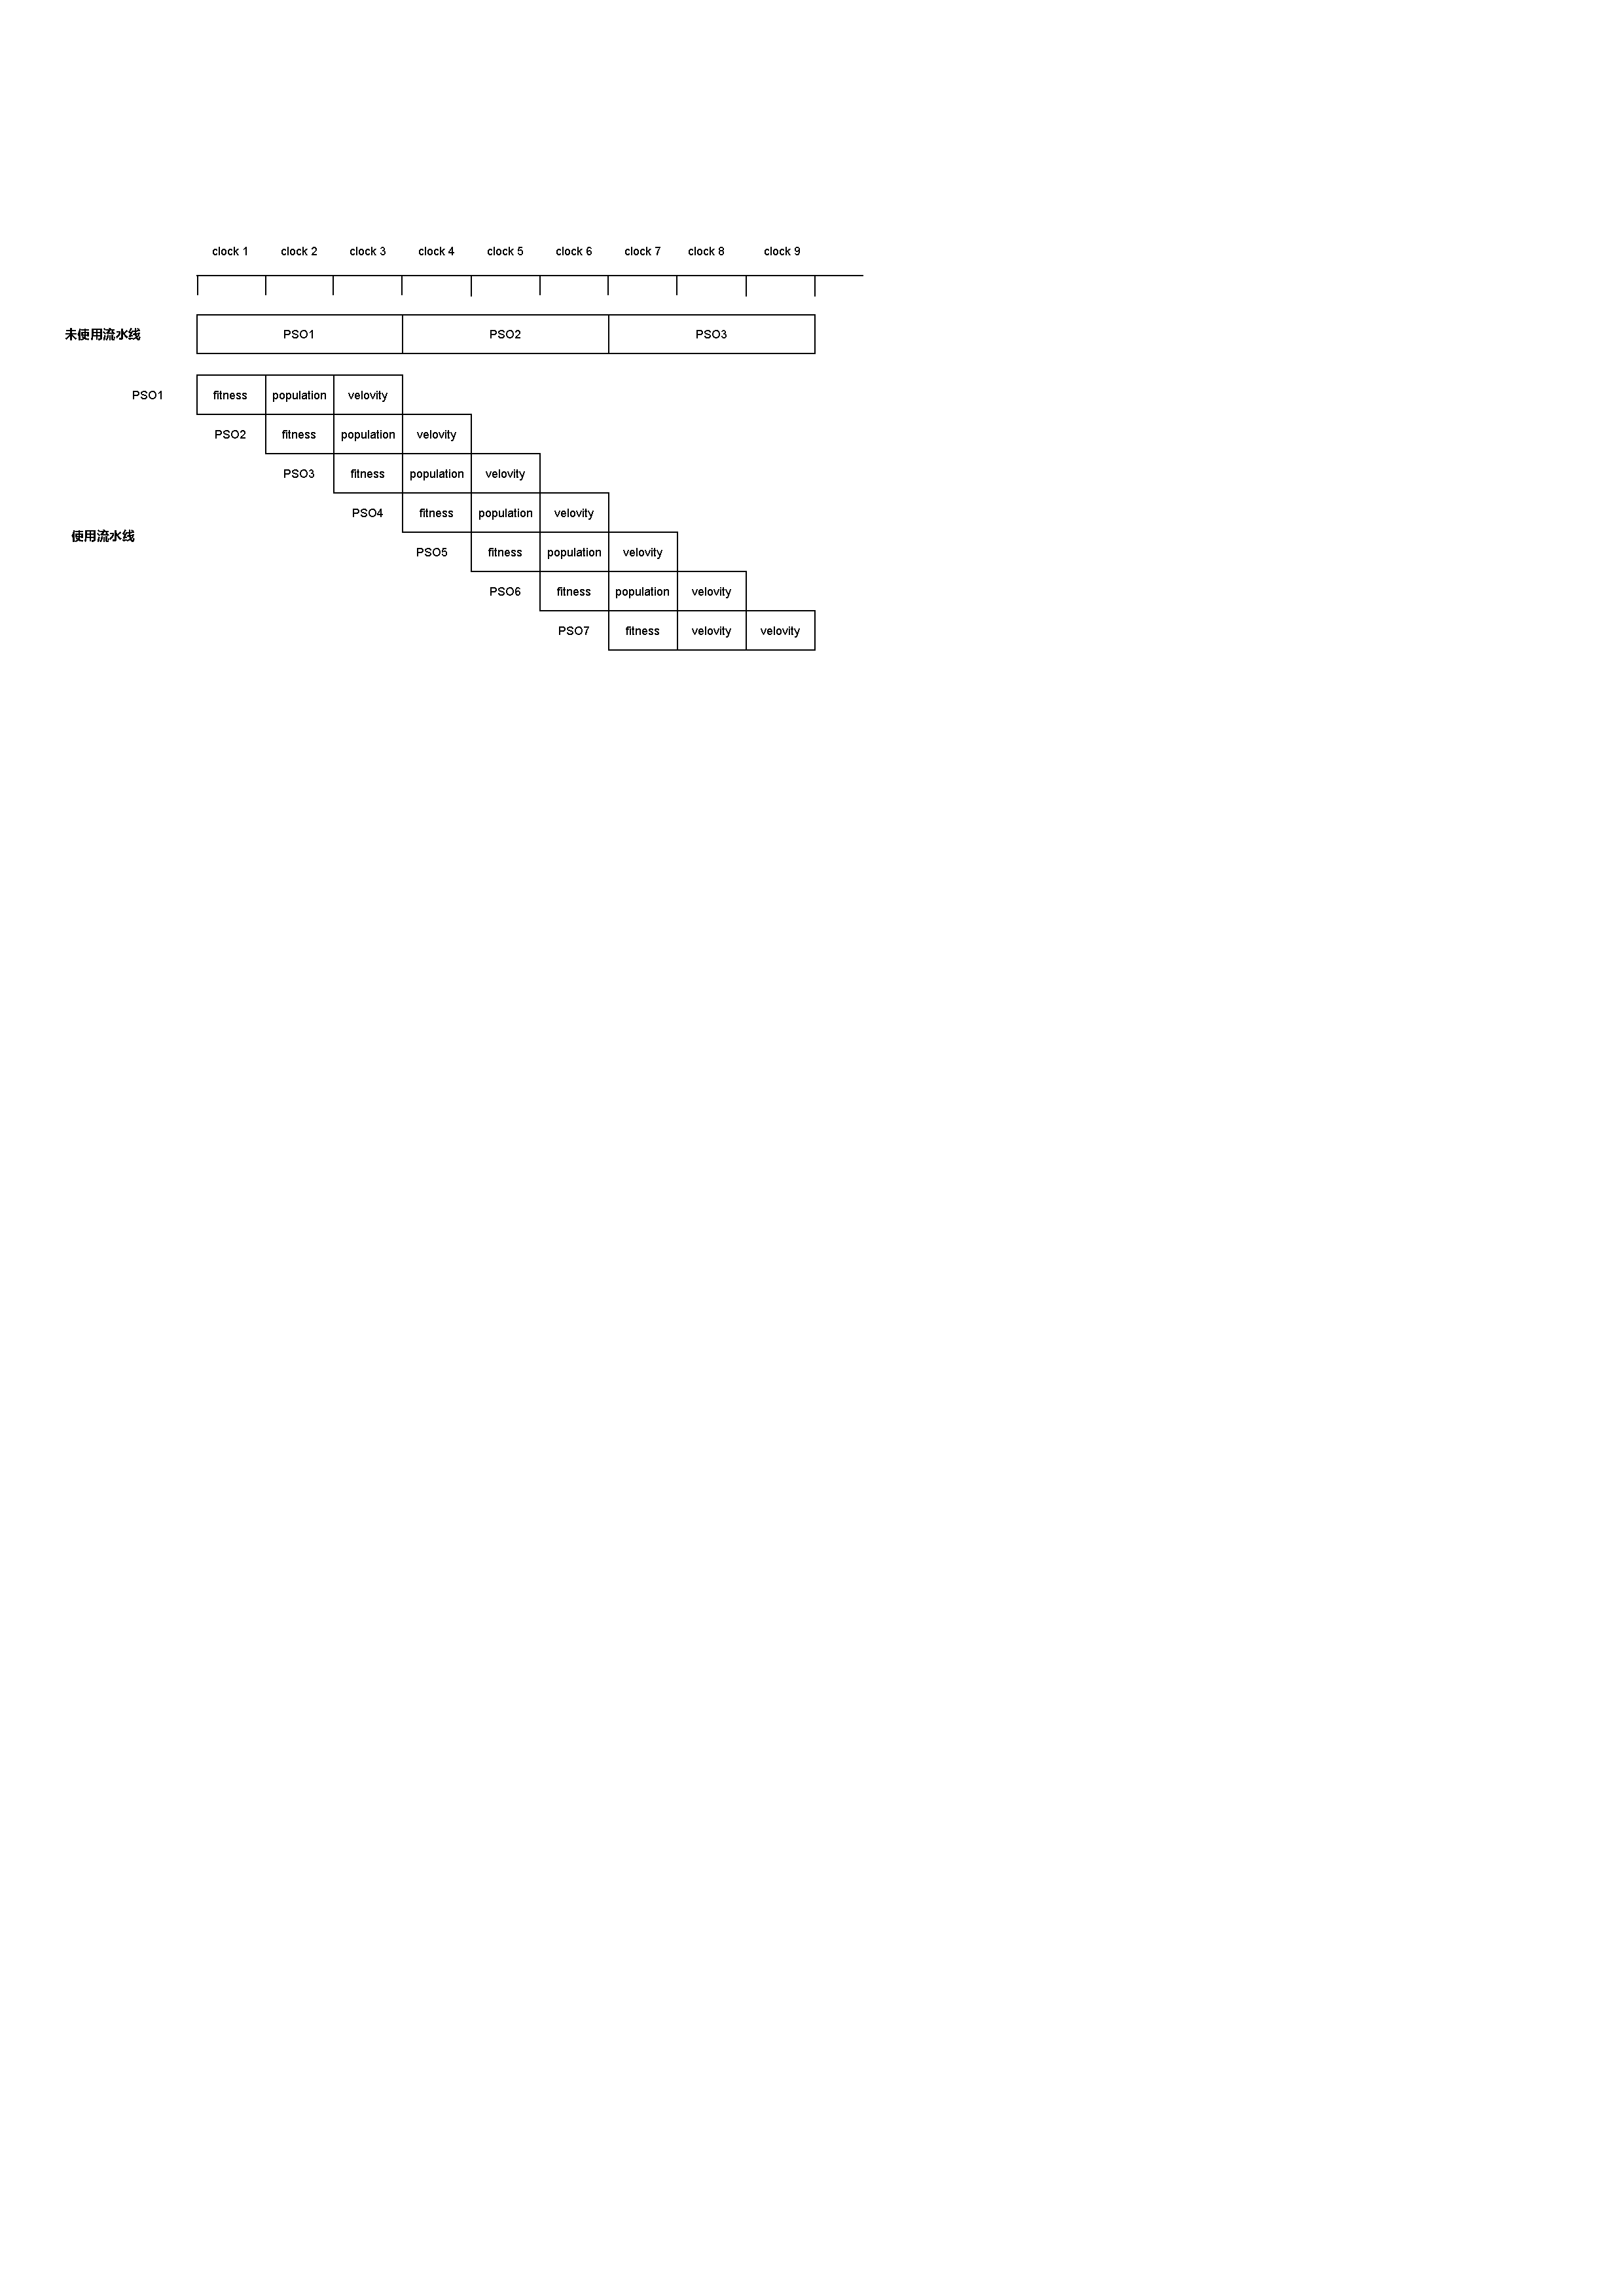
\includegraphics[width=14cm]{fig/5-fig/流水线示意图.drawio.pdf}
    \caption{流水线示意图}
    \label{fig:流水线示意图}
  \end{figure}

图\ref{fig:流水线示意图}画出了9个时钟周期内PSO操作情况,假设适应度计算(fitness)、速度和位置更新(velocity)以及种群信息更新(population)三个计算步骤需要的时间完全一致,都需要一个时钟周期,那么完成一次完整的PSO操作需要3个时钟周期。从图中可以看出,在未使用流水线技术时,9个时钟周期内只能完成3次PSO操作。如果采用了流水线技术,第一次PSO操作从第1个时钟周期开始,于第3个时钟周期完成,第二次PSO操作从第2个时钟周期开始,于第4个时钟周期结束,以此类推。可以看出在同一个时钟周期内,最多各只会有一次适应度计算、速度和位置更新以及种群信息更新,所以这不会引起硬件资源的冲突。采用流水线技术后,9个时钟周期内可以完成7次PSO操作,所以采用流水线技术可以很大程度上提升加速器的性能。

本文设计的用于干涉仪环境补偿的粒子群算法专用加速补偿系统为6级流水线,其中适应度计算模块由于含有大量乘法计算,所以设计为4级流水线,速度和位置更新以及种群信息更新模块乘法计算较少所以共为2级流水线。

\subsection{握手控制方案}
\label{握手控制方案}
由于采用了流水线技术,将一次PSO操作分成了多级流水完成,对于相邻的两级流水线,上一级的输出是下一级的输入,所以如果上一级的输出尚未准备好,那么下一级的流水线是无法进行计算的,需要被阻塞,直至上一级流水线的输出准备就绪;或者如果上一级的输出已经准备好了,但是下一级处于忙碌状态无法接收数据,那么上一级的输出是没法给下一级流水的,需要阻塞到下一级流水空闲了再把数据下发。上述这些情形导致相邻两级的流水需要一组控制信号进行通信,这样相邻的两级流水线才能知道自己什么时候能正常工作,这组信号就被称为握手信号\cite{LDPC解码器的异步流水线电路研究}。

本文设计的用于干涉仪环境补偿的粒子群算法加速补偿系统的握手控制方案中共含有4个握手信号:in$\_$vld、in$\_$rdy、out$\_$vld、out$\_$rdy,各信号含义如表\ref{tab:握手信号含义表}所示。如果两级流水线之间是直连的,无其他任何逻辑,那么通常上一级流水的out$\_$vld和out$\_$rdy分别连接的是本级流水的in$\_$vld、in$\_$rdy,当in$\_$vld、in$\_$rdy同时为高时称为完成一次握手,此时可认为上一级流水输出的信号已经被本级流水所暂存,上一级流水可以继续进行其他运算了,具体的时序图如图\ref{fig:握手控制模块时序图}所示。
\begin{table}[H]
    \centering
    \caption{握手信号含义表}
    \label{tab:握手信号含义表}
    \begin{tabular}{c|c|c}
        \hline
        名称                               & 含义                   &  信号流向         \\ \hline
        in$\_$vld              & 上一级流水的输出信号是否有效           &上一级流水$\rightarrow$本级流水        \\ \hline
        in$\_$rdy              & 否能接收上一级流水的信号              &本级流水  $\rightarrow$上一级流水       \\ \hline
        out$\_$vld             & 本级流水的输出信号是否有效            & 本级流水 $\rightarrow$下一级流水       \\ \hline
        out$\_$rdy             & 下一级流水能否接收信号                & 下一级流水$\rightarrow$本级流水       \\ \hline
    \end{tabular}
  \end{table}

\begin{figure}[htb]
    \centering
    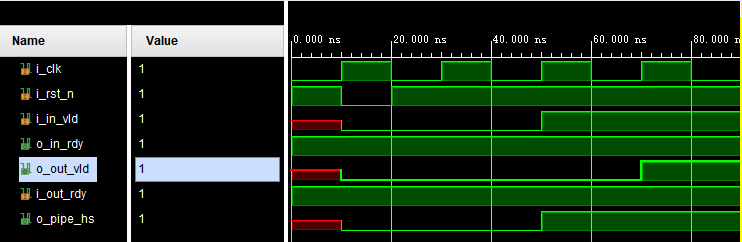
\includegraphics[width=14cm]{fig/5-fig/握手控制模块时序图.jpg}
    \caption{握手控制模块时序图}
    \label{fig:握手控制模块时序图}
\end{figure}

本文设计的流水线握手控制模块名称为pipe$\_$ctrl$\_$cell,其逻辑结构图为\ref{fig:握手控制模块逻辑结构图},其中i$\_$in$\_$vld即为上述的in$\_$vld信号,i表明这个信号对于pipe$\_$ctrl$\_$cell为输入信号(input),i$\_$rst$\_$n为模块的复位信号,i$\_$clk为模块的时钟信号,o$\_$pipe$\_$hs为成功握手信号。一个pipe$\_$ctrl$\_$cell模块需要的FPGA资源如表\ref{tab:握手控制模块资源消耗表}所示,主要使用到的资源为查找表(Look-Up-Table,简称LUT)以及寄存器。
\begin{figure}[htb]
    \centering
    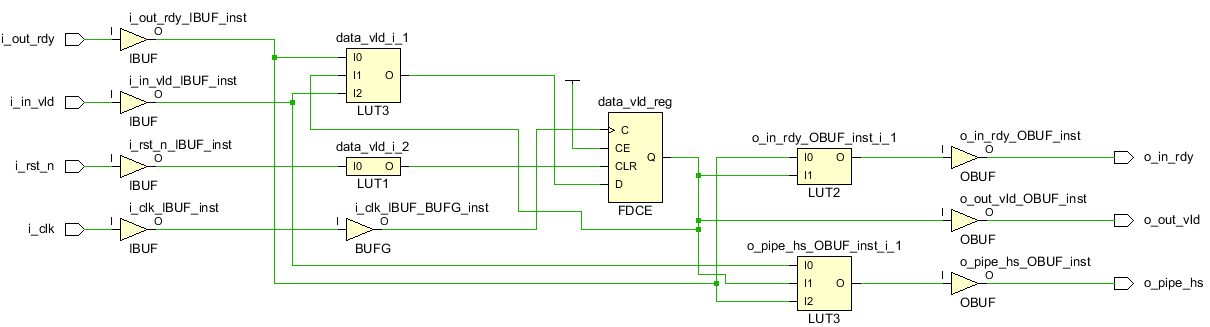
\includegraphics[width=14cm]{fig/5-fig/握手控制模块逻辑结构图.jpg}
    \caption{握手控制模块逻辑结构图}
    \label{fig:握手控制模块逻辑结构图}
  \end{figure}

  \begin{table}[H]
    \centering
    \caption{握手控制模块资源消耗表}
    \label{tab:握手控制模块资源消耗表}
    \begin{tabular}{c|c|c|c|c}
        \hline
        资源类别 & Slice LUTs & Slice Register & Bonded IOB & BUFGCTRL \\ \hline
        数量     & 3          & 1              & 7          & 1        \\ \hline
    \end{tabular}
  \end{table}

  \subsection{逻辑复制与资源共享技术}
  逻辑复制技术指的是在硬件设计的过程中,如果某级流水后负载过多,而且该处又为关键信号,就可以通过使用逻辑复制技术,将该处电路复制一份以降低该关键信号的扇出从而降低该关键信号的延迟,这样就可以提高电路的性能。在用于干涉仪环境补偿的粒子群算法加速补偿系统的设计过程中,如果设置的种群个体数过多,由式\eqref{eq:粒子群算法速度更新}和式\eqref{eq:粒子群算法位置新}可以看出在进行每个个体的速度位置更新时所需的$pbest_i$和$gbest$都来源于种群信息更新模块,这就会导致种群信息更新模块后的负载过多而使得其延迟过大,所以可以对其采用逻辑复制技术,采用逻辑复制技术前后如如图\ref{fig:逻辑复制技术示意图}所示。
  \begin{figure}[htb]
    \centering
    \subfigure[未使用逻辑复制]{
      \begin{minipage}[b]{0.99\textwidth}
        \centering
        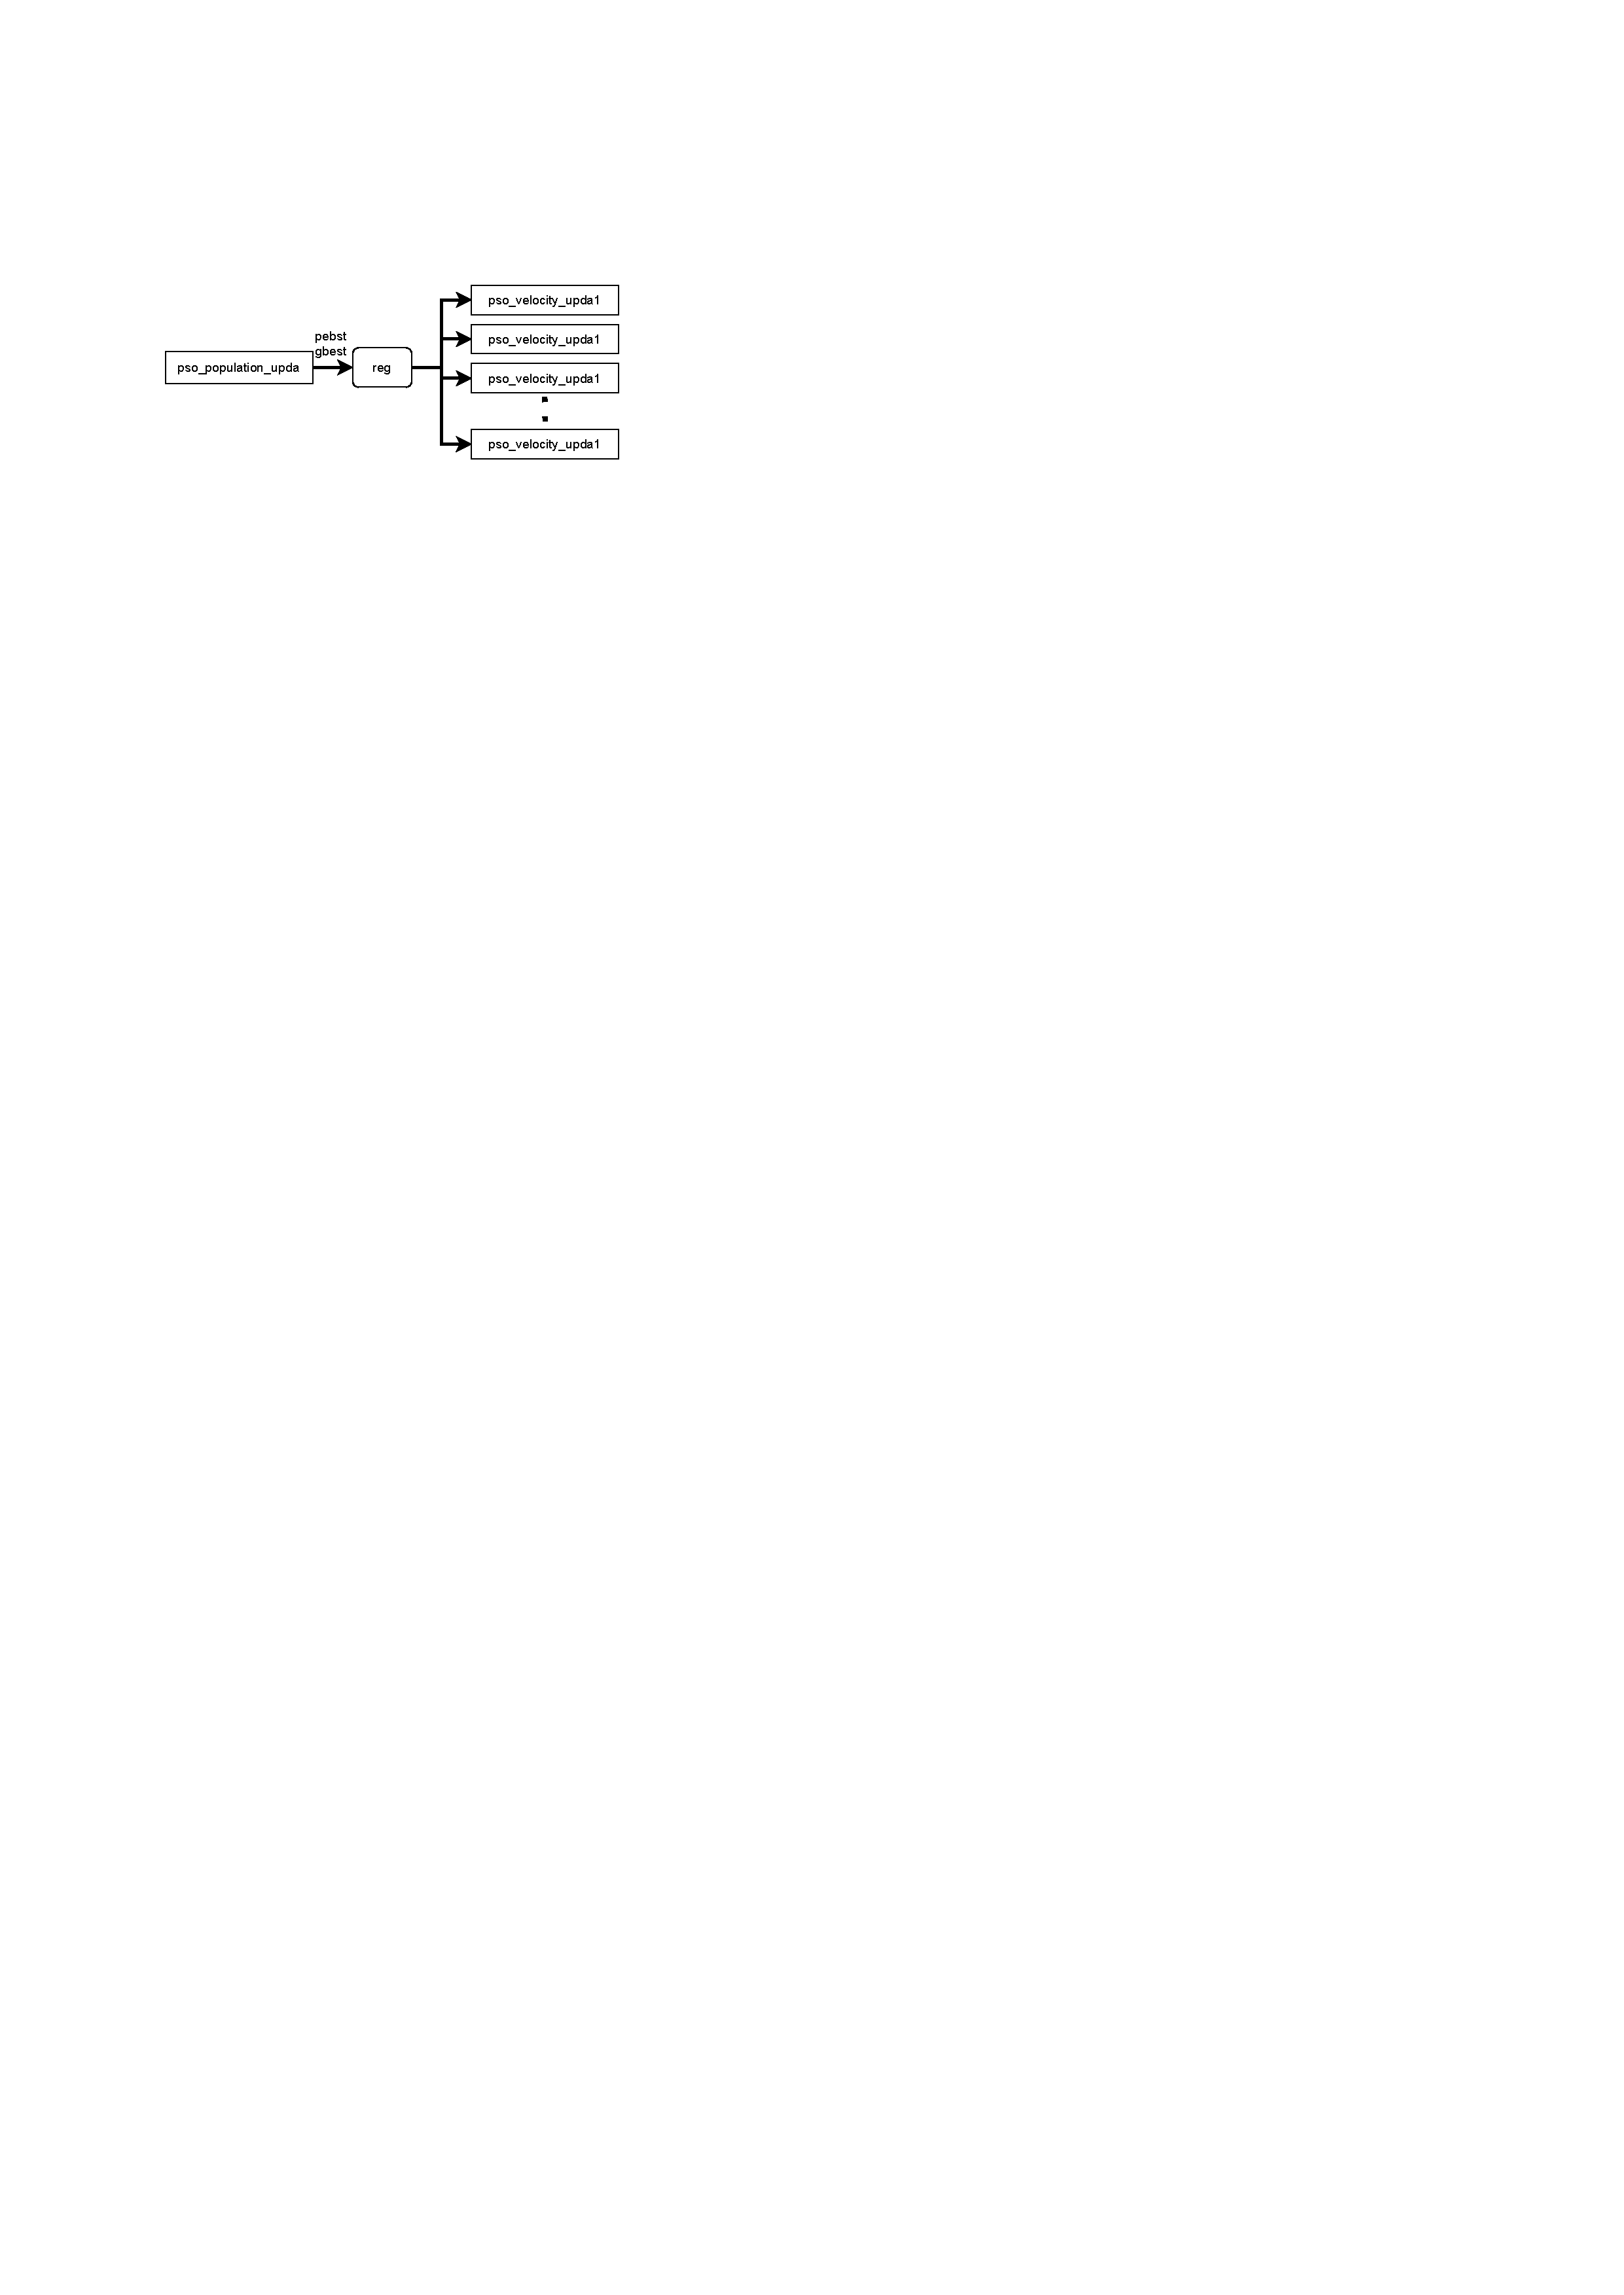
\includegraphics[width=8.5cm,height=3.3cm]{fig/5-fig/逻辑复制示意图a.drawio.pdf}
      \end{minipage}
      \label{fig:未使用逻辑复制}
    }
    \subfigure[使用逻辑复制]{
      \begin{minipage}[b]{0.99\textwidth}
        \centering
        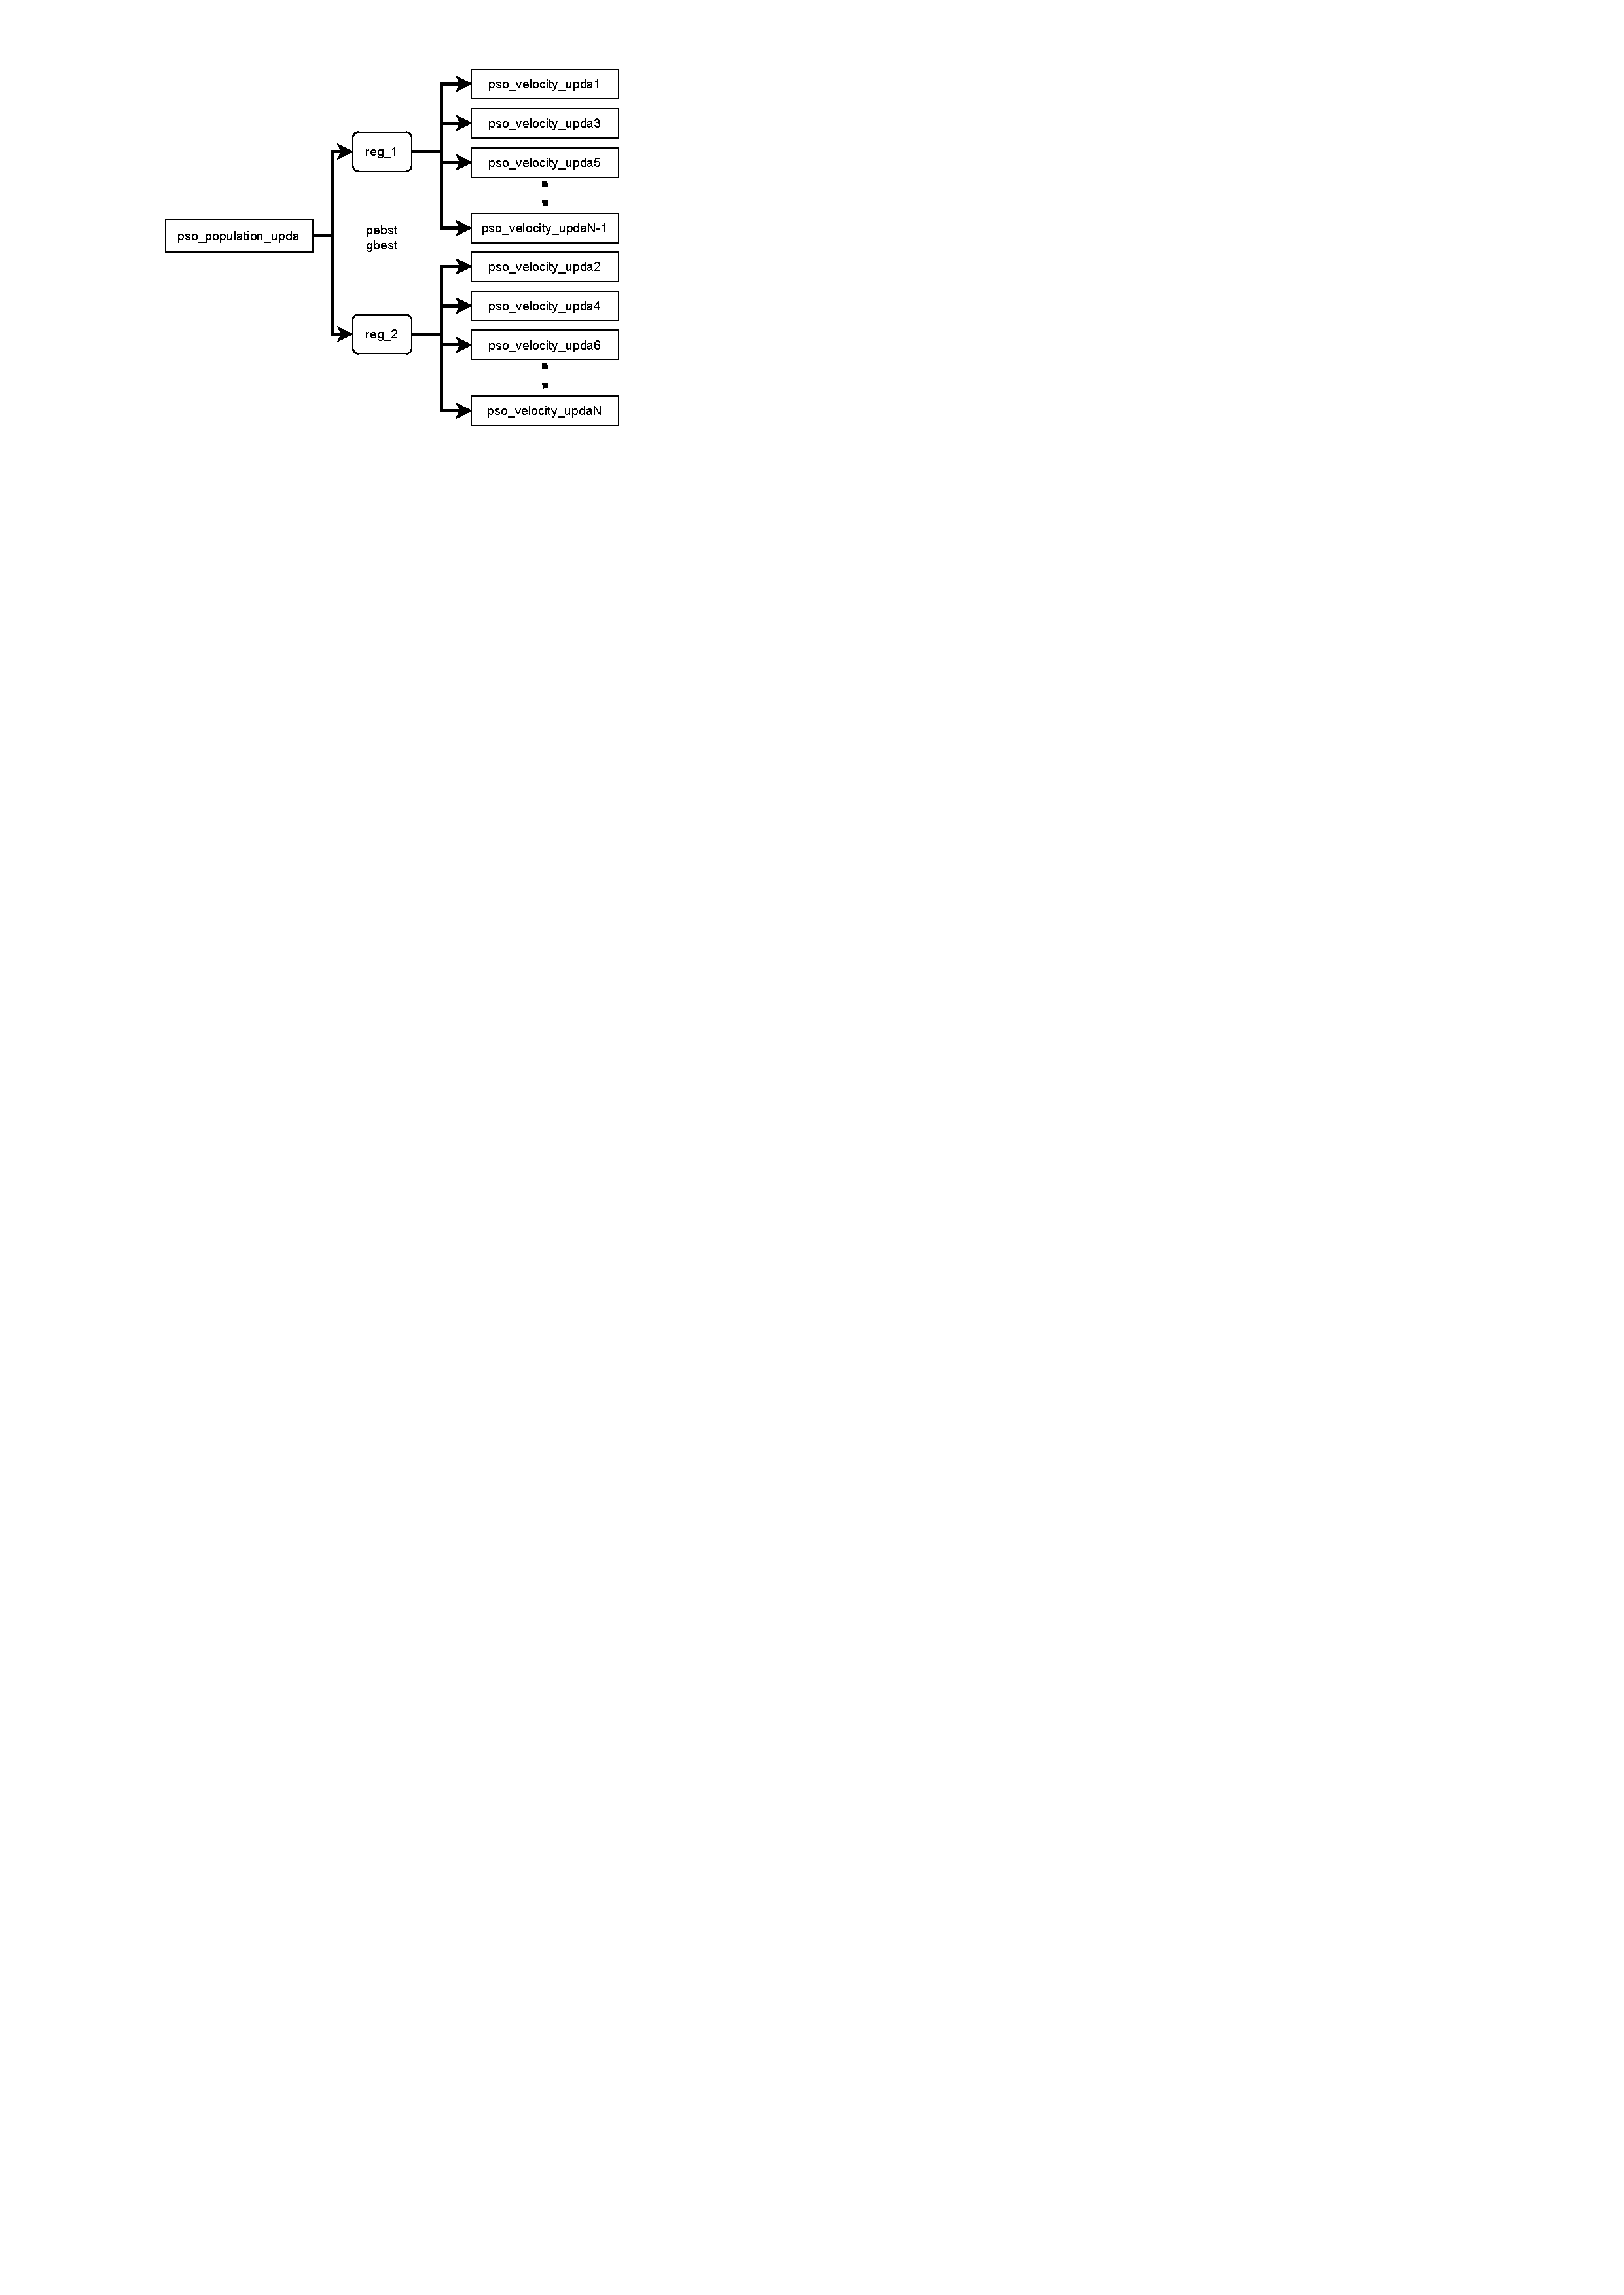
\includegraphics[width=8.8cm,height=6.6cm]{fig/5-fig/逻辑复制示意图b.drawio.pdf}
      \end{minipage}
      \label{fig:使用逻辑复制}
    }
    \caption{逻辑复制技术示意图}
    \label{fig:逻辑复制技术示意图}
  \end{figure}

  资源共享技术则是与逻辑复制技术相反,在不影响性能的非关键路径上,如果存在比较多的公共单元,则可以多个电路共同使用同一个公共单元,这么做可能会导致延时增大,但由于不是关键路径,所以影响较小,但这可以减小面积。

\subsection{门控时钟技术}
对于电路而言,其功耗主要分为两类:静态功耗的动态功耗。静态功耗又可以叫做待机功耗,它主要是由于电路中的漏电流导致的功耗,其计算公式如式\eqref{eq:静态功耗计算公式}所示,其中$I_s$为静态工作电流,$V_{DD}$为工作电压。而动态功耗又可以叫做开关功耗,它是由于逻辑翻转所产生的功耗,即电平发生$0\rightarrow1$和$1\rightarrow0$跳变时所产生的功耗,其计算方法如式\eqref{eq:动态功耗计算公式}所示,式中$C_L$为寄生电容,$S$为每个时钟周期内电路的平均翻转次数,$f_{clk}$为时钟频率。而由于现在FPGA的时钟频率一般为几十MHz到几百MHz,这意味着时钟每秒会发生几百万次到几千万次的跳变,所以由时钟翻转带来的功耗是很大的。减少这部分功耗最简单的方法就是:判断每个模块是否处于工作状态,如果不处于工作状态则将该模块的输入的时钟关闭,这种技术称为门控时钟技术。
\begin{equation}\label{eq:静态功耗计算公式}
    P_s = I_s \times V_{DD}.
    \end{equation}
\begin{equation}\label{eq:动态功耗计算公式}
    P_{dynamic}=SC_LV^2_{DD}f_{clk}.
    \end{equation}


为了判断每个模块是否处在工作状态,需要在每个模块的I/O中新增一个信号:busy,该信号为1代表该模块处于工作状态,为0则说明该模块处于空闲状态。有了busy信号之后,进行门控时钟的最简单的方法就是将busy信号和时钟信号clk相与,这样当模块处于空闲状态的时候,与门输出的结果就一直是0,就将时钟关断了,如果模块正在工作,busy信号为1,clk$\&$busy的结果仍然是clk,不会影响模块的正常工作。但是由于与门是电平逻辑,所以一旦busy信号有毛刺,就会导致经过门控时钟出来之后的时钟也有毛刺,而导致时钟信号错误的关断,这对电路的功能是致命的。所以当前门控时钟一般采用锁存门控或者寄存门控,这两种方法采用锁存器/寄存器对busy信号进行暂存,能很有效地避免毛刺造成干扰。本文使用锁存门控技术,其结构图和波形图如图\ref{fig:锁存门控的结构图和波形图}所示。$clk\_in$为原始时钟,$clk\_out$为经过时钟门控之后的模块输入时钟。
\begin{figure}[htb]
    \centering
    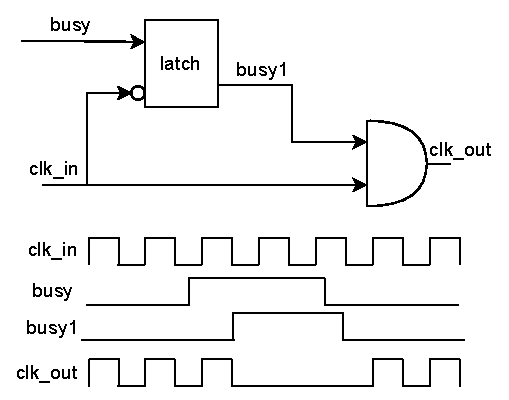
\includegraphics[width=8cm]{fig/5-fig/锁存门控的结构图和波形图.drawio.pdf}
    \caption{锁存门控的结构图和波形图}
    \label{fig:锁存门控的结构图和波形图}
\end{figure}

\subsection{随机数生成设计}
由于数字电路中只存在0和1两个值,并且要求任一时刻电路都处于确定的状态,并无中间态产生,否则会进入亚稳态,这导致对于数字电路而言,随机数的生成是一件非常困难的事情,电路生成的随机数大多都是伪随机数,即只在一定范围内进行随机,并且有规律可循。本文在随机数生成的设计上采用线性反馈移位寄存器(Linear Feedback Shift Register,简称LSFR),LSFR由若干个触发器和异或门组成,其原理是使用反馈函数改变LSFR中现存的序列,并将反馈函数的输出进行移位,从而在一定的序列长度内可以生成源源不断的伪随机输出。本文设计的随机数生成模块名称为pso$\_$lsfr$\_$rangen,其架构图如图\ref{fig:LSFR架构图}所示,这是一个8位的LSFR,反馈系数为101110001,所能产生的最大不重复序列的长度为$2^8-1=255$种,所以它能产生的最大255个随机值,并通过seed控制随机值的产生顺序。
\begin{figure}[htb]
    \centering
    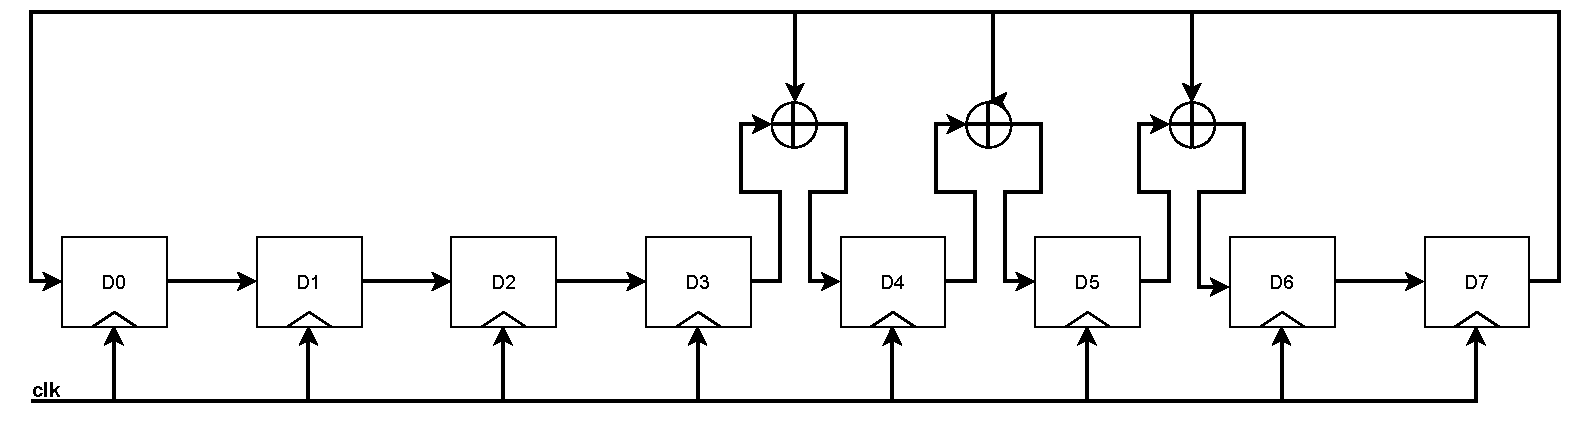
\includegraphics[width=14cm]{fig/5-fig/LSFR架构图.pdf}
    \caption{LSFR架构图}
    \label{fig:LSFR架构图}
\end{figure}

\section{粒子群算法加速补偿系统架构}
整个粒子群算法加速补偿系统架构如图\ref{fig:粒子群算法加速补偿系统架构示意图},其中pipe$\_$ctrl$\_$cell为\ref{握手控制方案}节中介绍的握手控制模块,pso$\_$fitness$\_$cal为适应度计算模块,并行放置了N个适应度计算模块,pso$\_$population$\_$upda为种群信息更新模块,pso$\_$velocity$\_$cal为速度和位置更新模块,也共放置了N个模块用于并行加速。

\begin{figure}[htb]
    \centering
    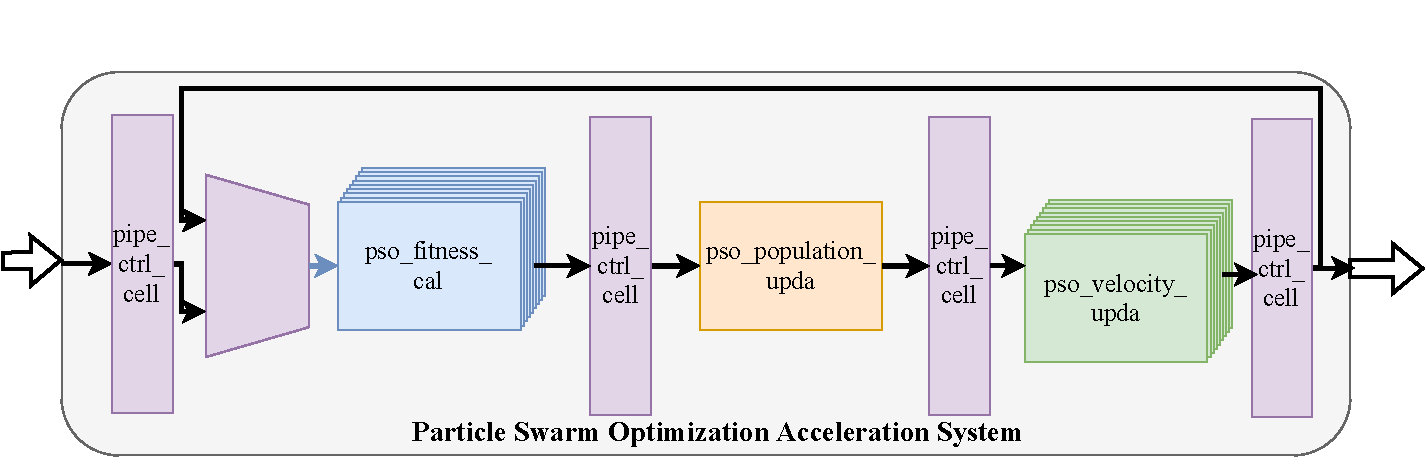
\includegraphics[width=14cm]{fig/5-fig/粒子群算法加速系统架构.drawio.pdf}
    \caption{粒子群算法加速补偿系统架构图}
    \label{fig:粒子群算法加速补偿系统架构示意图}
\end{figure}

为了兼顾硬件的灵活性和可维护性,某些可配置信息不使用寄存器配置方法,而采用parameter方法配置,具体参数含义及默认值如表\ref{tab:parameter定义表}所示。
\begin{table}[htb]
    \centering
    \caption{parameter定义表}
    \label{tab:parameter定义表}
        \begin{tabular}{c|c|c}
        \hline
        名称          & 含义                            & 默认值     \\ \hline
        SAM$\_$NUM    & 训练的样本数量,推荐为2的幂次方   & 128           \\ \hline
        IND$\_$NUM    & 种群的个体数量,推荐为2的幂次方   & 32            \\ \hline
        PARA$\_$NUM   & 待训练参数数量                  & 2      \\ \hline
        GEN$\_$NUM    & 迭代上限次数,推荐为2的幂次方    & 256       \\ \hline
        IW            & 整数部分位宽                    & 16      \\ \hline
        FW            & 小数部分位宽                    & 8     \\ \hline
    \end{tabular}
  \end{table}

整个粒子群算法加速补偿系统的接口信号如表\ref{tab:粒子群算法加速补偿系统接口信号表}所示,给出了顶层所有接口的名称、方向、位宽以及含义。其中$i\_$或$o\_$的前缀表明该信号是输入还是输出,$\_$cfg$\_$标志代表是一个寄存器接口,$\_$pso$\_$标志代表是系统的数据或控制信号输入,其余为系统的全局信号。
\begin{table}[htb]
    \centering
    \caption{粒子群算法加速补偿系统接口信号表}
    \label{tab:粒子群算法加速补偿系统接口信号表}
    \begin{tabular}{c|c|c|c}
        \hline
        接口名                                       & 接口方向  & 位宽               &含义                         \\ \hline
        i$\_$clk                                    & 输入      & 1                     & 系统时钟信号              \\ \hline
        i$\_$rst$\_$n                               & 输入      & 1                     & 系统复位信号   \\ \hline
        i$\_$flush                                  & 输入      & 1                     & 系统刷新信号              \\ \hline
        i$\_$cfg$\_$pso$\_$in$\_$initial$\_$para    & 输入      & PARA$\_$NUM*(IW+FW)   & 训练起点                 \\ \hline
        i$\_$cfg$\_$pso$\_$in$\_$initial$\_$lastv   & 输入      & PARA$\_$NUM*(IW+FW)   & 训练的初始速度            \\ \hline
        i$\_$cfg$\_$pso$\_$in$\_$len                & 输出      & 8                     & 测量臂长度                \\ \hline
        i$\_$cfg$\_$pso$\_$start                    & 输入      & 1                     & 系统开始信号              \\ \hline
        o$\_$cfg$\_$pso$\_$busy                     & 输出      & 1                     & 系统忙碌标志位            \\ \hline
        o$\_$cfg$\_$pso$\_$done                     & 输出      & 1                     & 计算完成信号              \\ \hline
        i$\_$pso$\_$in$\_$vld                       & 输入      & 1                     & 有效信号            \\ \hline
        o$\_$pso$\_$in$\_$rdy                       & 输出      & 1                     & 接收准备信号          \\ \hline
        i$\_$pso$\_$in$\_$sample$\_$temp            & 输入      & SAM$\_$NUM*(IW+FW)    & 温度数据            \\ \hline
        i$\_$pso$\_$in$\_$sample$\_$pres            & 输入      & SAM$\_$NUM*(IW+FW)    & 气压数据            \\ \hline
        i$\_$pso$\_$in$\_$sample$\_$disp            & 输入      & SAM$\_$NUM*(IW+FW)    & 位移数据            \\ \hline
        o$\_$pso$\_$out$\_$vld                      & 输出      & 1                     & 有效信号            \\ \hline
        i$\_$pso$\_$out$\_$rdy                      & 输入      & 1                     & 接收准备信号          \\ \hline
        o$\_$pso$\_$trained$\_$temp                 & 输出      & (IW+FW)               & 温度因子          \\ \hline
        o$\_$pso$\_$trained$\_$pres                 & 输出      & (IW+FW)               & 气压因子          \\ \hline
    \end{tabular}
  \end{table}

\subsection{适应度计算模块架构}
适应度计算模块的架构如图\ref{fig:适应度计算模块架构图}所示的四级流水结构,图中也画出了大致的数据流,其中refractive$\_$cal为折射率计算,其计算方法如式\eqref{eq:线性形式的Edlen公式},compensation $\_$value为补偿值计算,其计算方法如式\eqref{eq:环境误差公式};error$\_$cal为适应度计算,其计算方法跟式\eqref{eq:均方根误差计算公式}类似,但是由于数字电路比较难实现算数平方根操作,所以将式中的算术平方根变为绝对值。要实现绝对值操作需要用到多个比较器,首先需要判断两个数符号位的关系,然后再判断数值位的大小关系,结合两次判断的结果得出两个数之间的大小关系,然后进行减法以实现绝对值操作。reg则代表相邻两级相邻流水线之间暂存数据的寄存器堆,虚线框表示的monitor为监视器,主要是为适应度计算模块每级流水验证时提供比对值。
  \begin{figure}[htb]
    \centering
    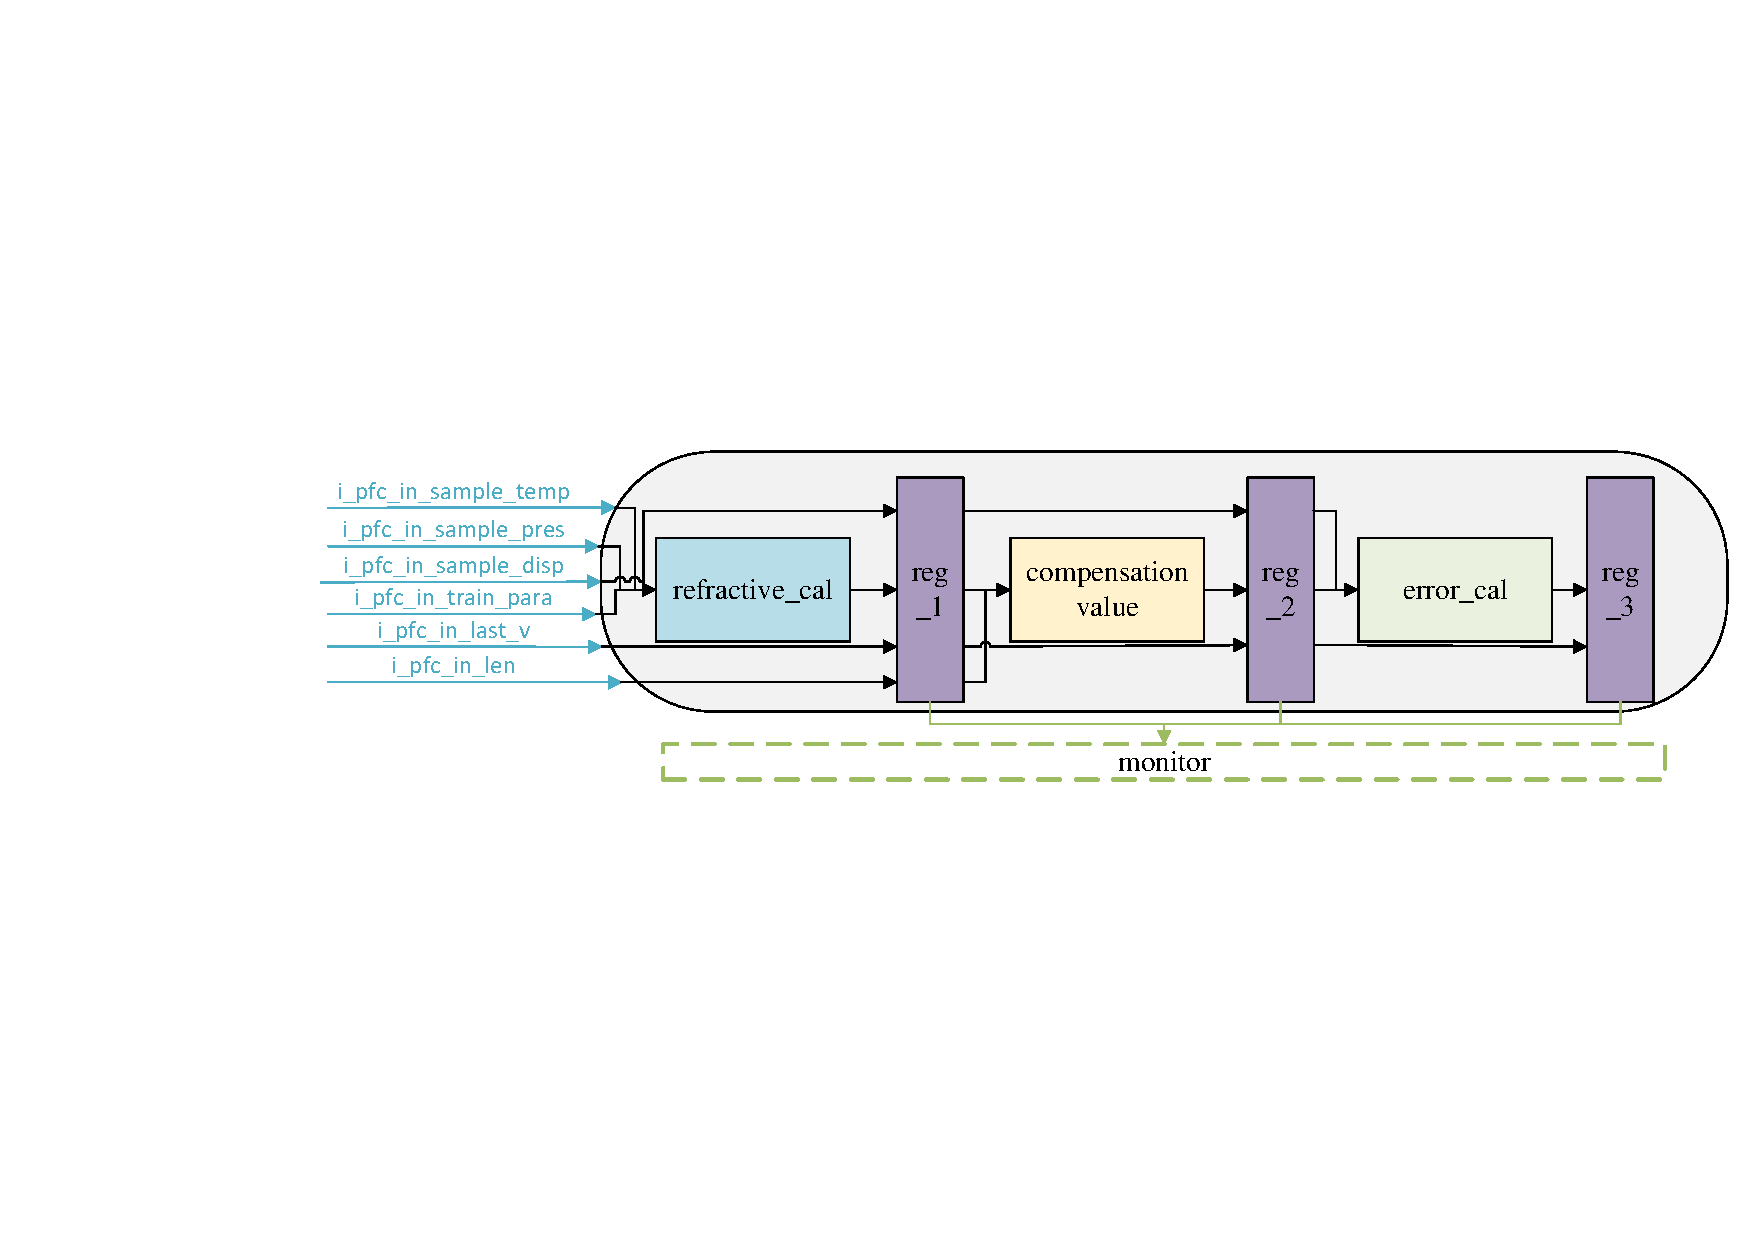
\includegraphics[width=14cm]{fig/5-fig/适应度计算模块架构图.pdf}
    \caption{适应度计算模块架构图}
    \label{fig:适应度计算模块架构图}
\end{figure}

适应度计算模块的所有接口信号如表\ref{tab:适应度计算模块接口信号表}所示,其中pfc为pso$\_$fitness$\_$cal的缩写首字母,标志着该信号为适应度计算模块的接口。
\begin{table}[htb]
    \centering
    \caption{适应度计算模块接口信号表}
    \label{tab:适应度计算模块接口信号表}
    \begin{tabular}{c|c|c|c}
        \hline
        接口名                               & 接口方向  & 位宽               &含义                        \\ \hline
        i$\_$clk                            & 输入      & 1                     & 时钟信号             \\ \hline
        i$\_$rst$\_$n                       & 输入      & 1                     & 复位信号             \\ \hline
        i$\_$flush                          & 输入      & 1                     & 刷新信号             \\ \hline
        i$\_$pfc$\_$in$\_$vld               & 输入      & 1                     & 有效信号        \\ \hline
        o$\_$pfc$\_$in$\_$rdy               & 输出      & 1                     & 准备信号        \\ \hline
        i$\_$pfc$\_$in$\_$sample$\_$temp    & 输入      & SAM$\_$NUM*(IW+FW)    & 温度数据        \\ \hline
        i$\_$pfc$\_$in$\_$sample$\_$pres    & 输入      & SAM$\_$NUM*(IW+FW)    & 气压数据        \\ \hline
        i$\_$pfc$\_$in$\_$sample$\_$disp    & 输入      & SAM$\_$NUM*(IW+FW)    & 位移数据        \\ \hline
        i$\_$pfc$\_$in$\_$train$\_$para     & 输入      & PARA$\_$NUM*(IW+FW)   & 当前训练参数     \\ \hline
        i$\_$pfc$\_$in$\_$last$\_$v         & 输入      & PARA$\_$NUM*(IW+FW)   & 当前速度        \\ \hline
        i$\_$pfc$\_$in$\_$len               & 输入      & 8                     & 测量臂长度      \\ \hline
        o$\_$pfc$\_$out$\_$vld              & 输出      & 1                     & 有效信号        \\ \hline
        i$\_$pfc$\_$out$\_$rdy              & 输入      & 1                     & 准备信号        \\ \hline
        o$\_$pfc$\_$out$\_$busy             & 输出      & 1                     & 工作标志位            \\ \hline
        o$\_$pfc$\_$out$\_$train$\_$para    & 输出      & PARA$\_$NUM*(IW+FW)   & 当前训练参数     \\ \hline
        o$\_$pfc$\_$out$\_$last$\_$v        & 输出      & PARA$\_$NUM*(IW+FW)   & 当前速度         \\ \hline
        o$\_$pfc$\_$out$\_$fitness          & 输出      & IW+IW+FW+8            & 适应度结果       \\ \hline
    \end{tabular}
  \end{table}

\subsection{种群信息更新模块架构}
种群信息更新模块的架构如图\ref{fig:适应度计算模块架构图}所示,为两级流水结构并画出了大致的数据流。其中32to1是找出32个个体适应度最小的一个,得到该个体对应的两个训练参数,其结构为5级比较器,其中第一级有16个二选一的比较器,从32组数据中找出较小的16组数据,第二级有8个二选一比较器,第三级有4个,以此类推,在最后一级比较器的输出即可选中32组数据中个体适应度最小的一组。

global$\_$upda是比较32to1中找出的最小适应度值,跟模块本身记录的最小适应度值相比较,如果32to1中的适应度小,则将模块记录的适应度值进行更新;person$\_$upda是将32个种群个体分开判断,比较当前周期的计算的适应度值是否比模块自身的记录的适应值小,如果小则进行更新。global$\_$upda和person$\_$upda都是使用一个寄存器和一个比较器组合搭建的。reg则代表相邻两级相邻流水线之间暂存数据的寄存器堆,虚线框表示的monitor为监视器,主要是用于验证时提供比对值。
\begin{figure}[htb]
    \centering
    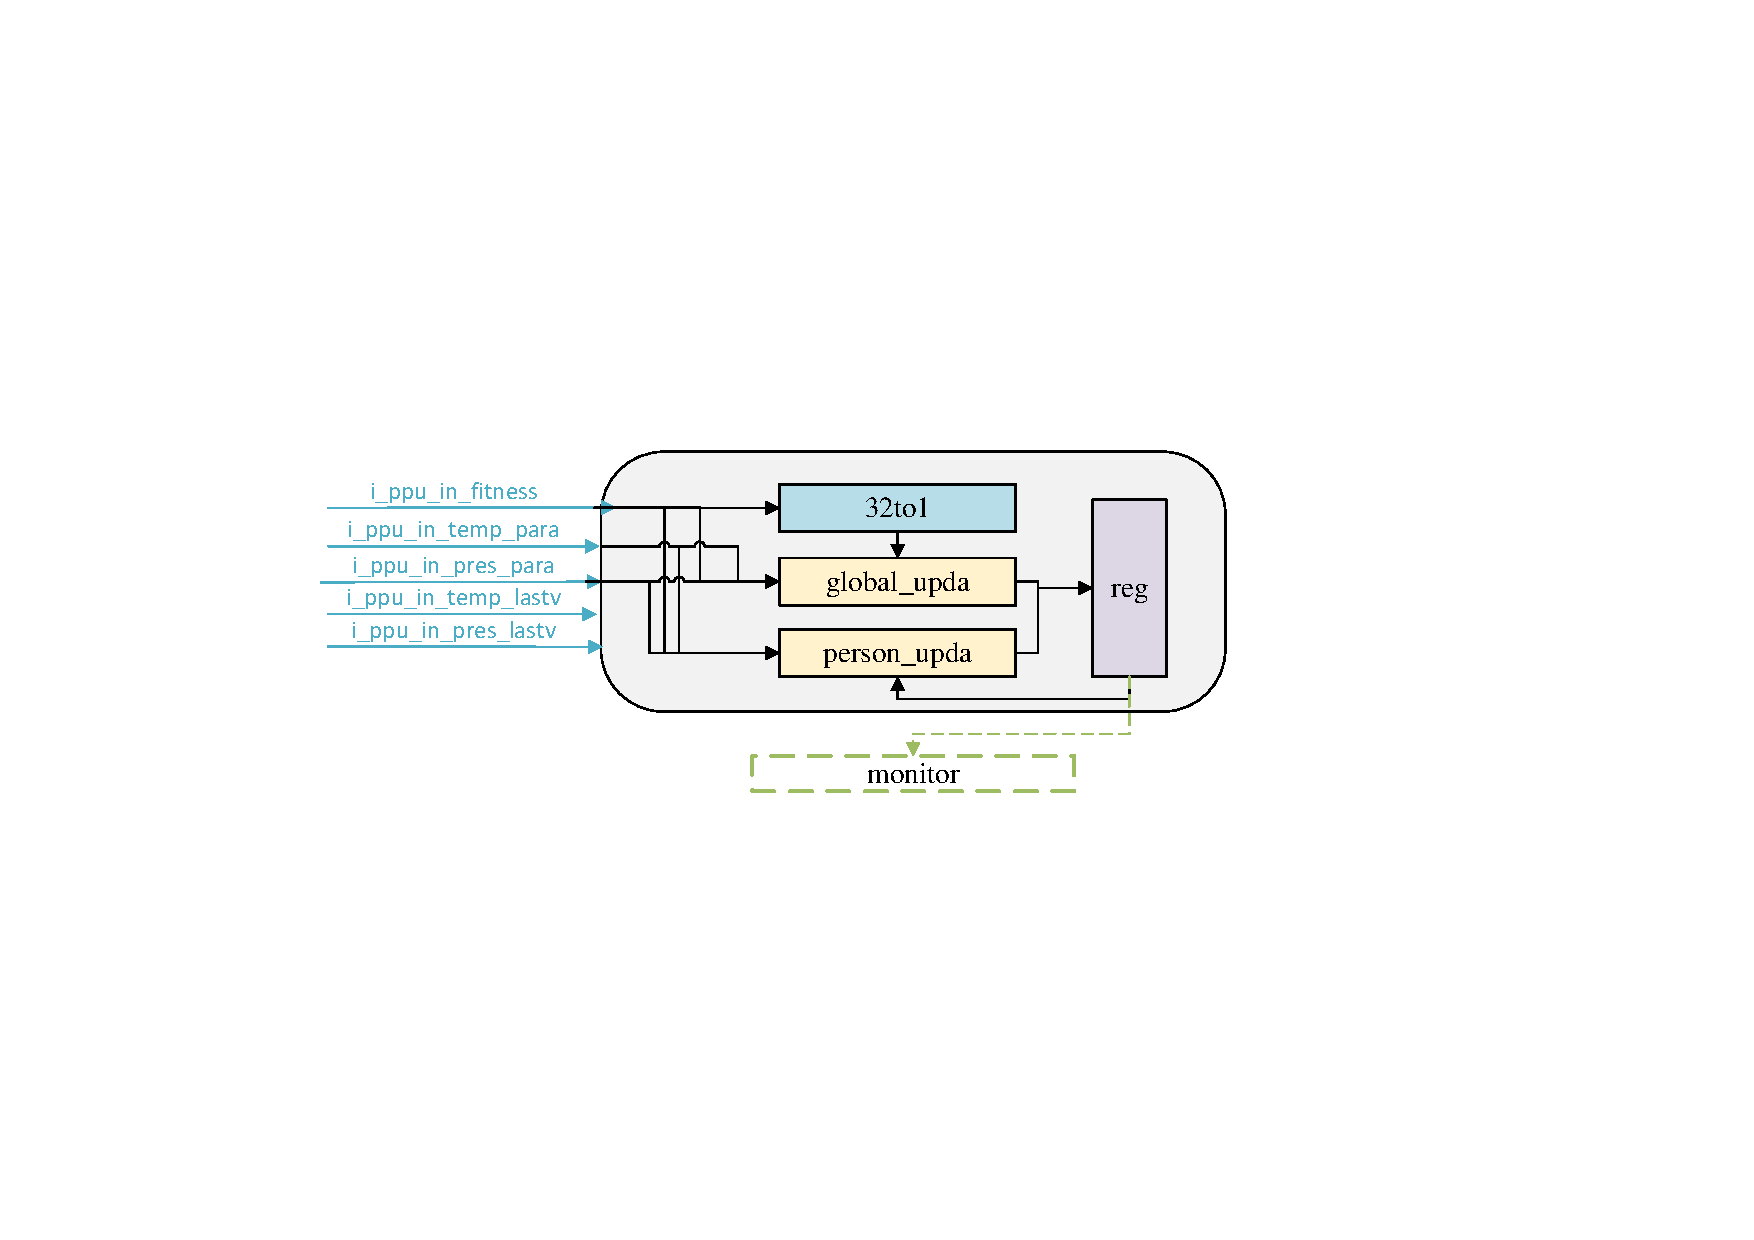
\includegraphics[width=12cm]{fig/5-fig/种群信息更新模块架构.pdf}
    \caption{种群信息更新模块架构}
    \label{fig:种群信息更新模块架构}
\end{figure}

种群信息更新模块的所有接口信号如表\ref{tab:种群信息更新模块接口信号表}所示,其中ppu为pso$\_$population$\_$upda的缩写首字母,标志着该信号为种群信息更新模块的接口。
\begin{table}[htb]
    \centering
    \caption{种群信息更新模块接口信号表}
    \label{tab:种群信息更新模块接口信号表}
    \begin{tabular}{c|c|c|c}
        \hline
        接口名                               & 接口方向  & 位宽               &含义                        \\ \hline
        i$\_$clk                                       & 输入      & 1                     & 时钟信号             \\ \hline
        i$\_$rst$\_$n                                  & 输入      & 1                     & 复位信号             \\ \hline
        i$\_$flush                                     & 输入      & 1                     & 刷新信号             \\ \hline
        i$\_$ppu$\_$in$\_$vld                          & 输入      & 1                     & 有效信号        \\ \hline
        o$\_$ppu$\_$in$\_$rdy                          & 输出      & 1                     & 准备信号        \\ \hline
        i$\_$ppu$\_$in$\_$fitness                      & 输入      & IND$\_$NUM*(2IW+FW+8) & 适应度          \\ \hline
        i$\_$ppu$\_$in$\_$temp$\_$para                 & 输入      & IND$\_$NUM*(IW+FW)    & 温度参数        \\ \hline
        i$\_$ppu$\_$in$\_$pres$\_$para                 & 输入      & IND$\_$NUM*(IW+FW)    & 气压参数        \\ \hline
        i$\_$ppu$\_$in$\_$temp$\_$lastv                & 输入      & IND$\_$NUM*(IW+FW)    & 温度速度        \\ \hline
        i$\_$ppu$\_$in$\_$pres$\_$lastv                & 输入      & IND$\_$NUM*(IW+FW)    & 气压速度       \\ \hline

        o$\_$ppu$\_$out$\_$vld                         & 输出      & 1                     & 有效信号        \\ \hline
        i$\_$ppu$\_$out$\_$rdy                         & 输入      & 1                     & 准备信号        \\ \hline
        o$\_$ppu$\_$out$\_$temp$\_$para                & 输出      & IND$\_$NUM*(IW+FW)    & 温度参数        \\ \hline
        o$\_$ppu$\_$out$\_$pres$\_$para                & 输出      & IND$\_$NUM*(IW+FW)    & 气压参数        \\ \hline
        o$\_$ppu$\_$out$\_$temp$\_$lastv               & 输出      & IND$\_$NUM*(IW+FW)    & 温度速度        \\ \hline
        o$\_$ppu$\_$out$\_$pres$\_$lastv               & 输出      & IND$\_$NUM*(IW+FW)    & 气压速度        \\ \hline
        o$\_$ppu$\_$out$\_$global$\_$temp              & 输出      & (IW+FW)               & 全局最优温度        \\ \hline
        o$\_$ppu$\_$out$\_$global$\_$pres              & 输出      & (IW+FW)               & 全局最优气压        \\ \hline
        o$\_$ppu$\_$out$\_$person$\_$temp              & 输出      & IND$\_$NUM*(IW+FW)    & 个体最优温度        \\ \hline
        o$\_$ppu$\_$out$\_$person$\_$pres              & 输出      & IND$\_$NUM*(IW+FW)    & 个体最优气压        \\ \hline
    \end{tabular}
  \end{table}

\subsection{速度和位置更新模块架构}
速度和位置更新模块架构的架构如图\ref{fig:速度和位置更新模块架构图}所示的两级流水结构,图中也画出了大致的数据流。其中LSFR1和LSFR2为2个8位的线性反馈移位寄存器,用于产生式\eqref{eq:粒子群算法速度更新}中的两个随机数,velocity$\_$upda和position$\_$upda分别为计算式\eqref{eq:粒子群算法速度更新}和\eqref{eq:粒子群算法位置新}。reg则代表相邻两级相邻流水线之间暂存数据的寄存器堆,虚线框表示的monitor为监视器,主要是用于验证时提供比对值。
\begin{figure}[htb]
    \centering
    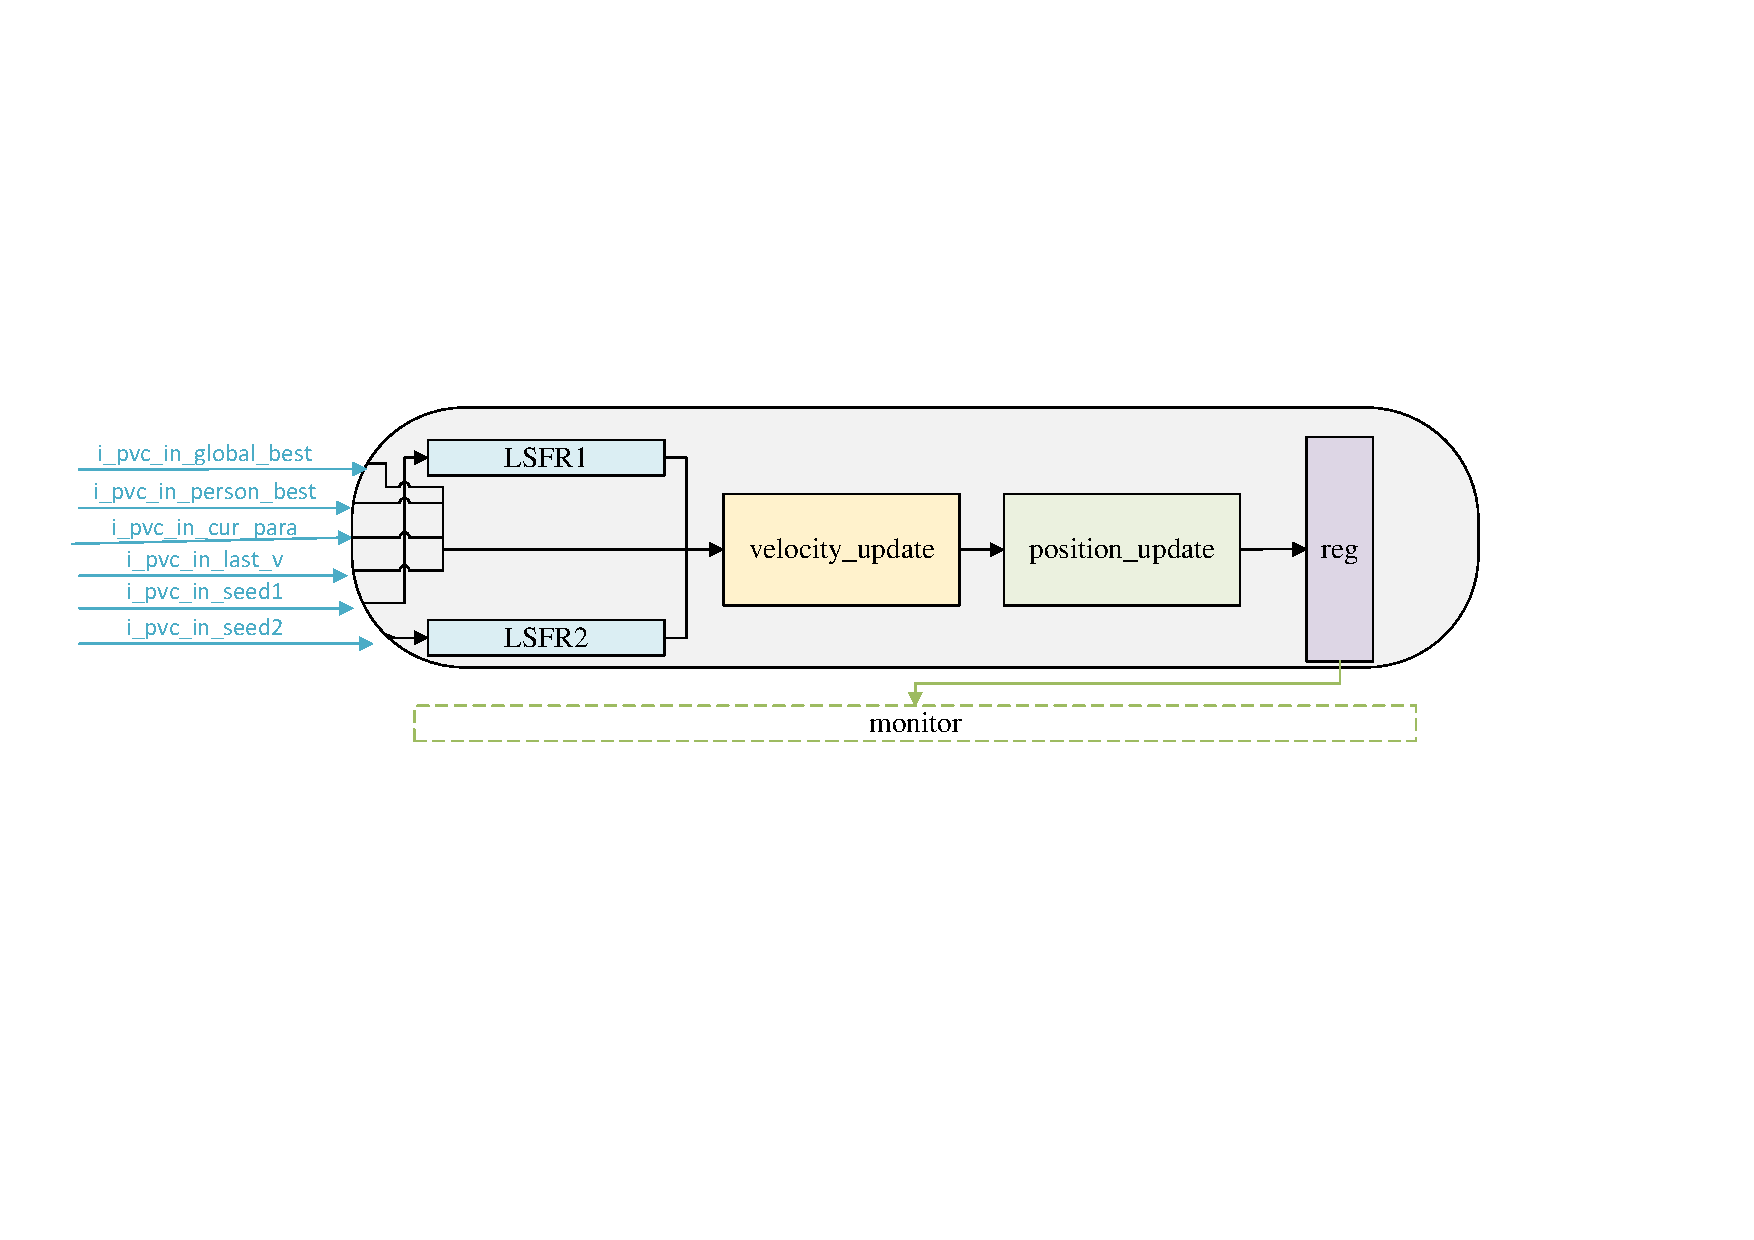
\includegraphics[width=14cm,height=5cm]{fig/5-fig/速度和位置更新模块架构图.pdf}
    \caption{速度和位置更新模块架构图}
    \label{fig:速度和位置更新模块架构图}
\end{figure}

速度和位置更新模块的所有接口信号如表\ref{tab:速度和位置更新模块接口信号表}所示,其中pvc为pso$\_$velocity$\_$cal的缩写首字母,标志着该信号为速度和位置更新模块的接口。

\begin{table}[htb]
    \centering
    \caption{速度和位置更新模块接口信号表}
    \label{tab:速度和位置更新模块接口信号表}
\begin{tabular}{c|c|c|c}
    \hline
    接口名                                          & 接口方向  & 位宽               &含义                        \\ \hline
    i$\_$clk                                       & 输入      & 1                     & 时钟信号             \\ \hline
    i$\_$rst$\_$n                                  & 输入      & 1                     & 复位信号             \\ \hline
    i$\_$flush                                     & 输入      & 1                     & 刷新信号             \\ \hline
    i$\_$pvc$\_$in$\_$vld                          & 输入      & 1                     & 有效信号        \\ \hline
    o$\_$pvc$\_$in$\_$rdy                          & 输出      & 1                     & 准备信号        \\ \hline
    i$\_$pvc$\_$in$\_$cur$\_$para                  & 输入      & PARA$\_$NUM*(IW+FW)   & 当前训练参数         \\ \hline
    i$\_$pvc$\_$in$\_$global$\_$temp               & 输出      & (IW+FW)               & 全局最优温度参数        \\ \hline
    i$\_$pvc$\_$in$\_$global$\_$pres               & 输出      & (IW+FW)               & 全局最优气压参数        \\ \hline
    i$\_$pvc$\_$in$\_$person$\_$temp               & 输出      & IND$\_$NUM*(IW+FW)    & 个体最优温度参数        \\ \hline
    i$\_$pvc$\_$in$\_$person$\_$pres               & 输出      & IND$\_$NUM*(IW+FW)    & 个体最优气压参数        \\ \hline
    i$\_$pvc$\_$in$\_$lsfr$\_$seed1                & 输入      & 8                     & 随机种子              \\ \hline
    i$\_$pvc$\_$in$\_$lsfr$\_$seed2                & 输入      & 8                     & 随机种子              \\ \hline


    o$\_$pvc$\_$out$\_$vld                         & 输出      & 1                     & 有效信号        \\ \hline
    i$\_$pvc$\_$out$\_$rdy                         & 输入      & 1                     & 准备信号        \\ \hline
    o$\_$pfc$\_$out$\_$nxt$\_$para                 & 输出      & PARA$\_$NUM*(IW+FW)   & 更新训练参数     \\ \hline
    o$\_$pfc$\_$out$\_$nxt$\_$v                    & 输出      & PARA$\_$NUM*(IW+FW)   & 更新速度         \\ \hline

\end{tabular}
\end{table}

\subsection{多起点训练方法及寄存器配置}
常规的粒子群算法一般都是单起点训练的,但是由于本文提出的温度梯度的分段式粒子群算法补偿方法中在温度变化梯度过大触发一次分段训练时,采用的粒子群算法的训练起点是上一次的训练的训练结果,如\ref{温度梯度的分段式粒子群算法补偿方法}节所述,这就导致了设计的粒子群加速补偿系统需要支持多起点训练,同时在\ref{流水线技术}节中也说明了整个粒子群算法加速补偿系统是一个6级流水线的设计,如果只用1个起点进行训练是无法覆盖整个流水线的初始延迟,其波形如图\ref{fig:单起点训练时序图}所示。
\begin{figure}[htb]
    \centering
    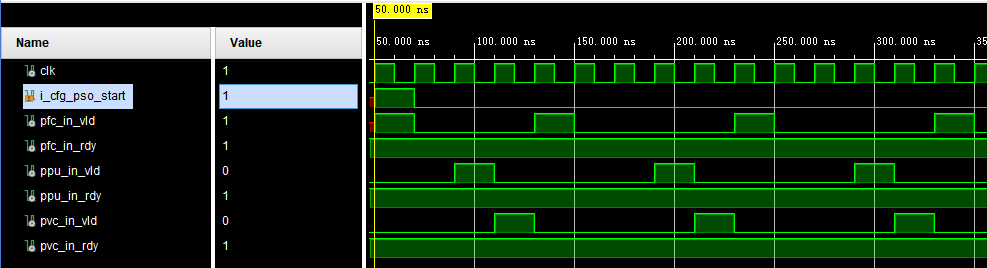
\includegraphics[width=14cm]{fig/5-fig/单起点训练时序图.jpg}
    \caption{单起点训练时序图}
    \label{fig:单起点训练时序图}
\end{figure}

从图中可以看出由于流水线较深使得如果只从一个起点开始训练,每个模块仍然有较长的空闲状态,硬件的利用率较低,这与流水线设计的初衷相悖,所以采用多起点进行训练则可以很好地解决这个问题。
\begin{figure}[htb]
    \centering
    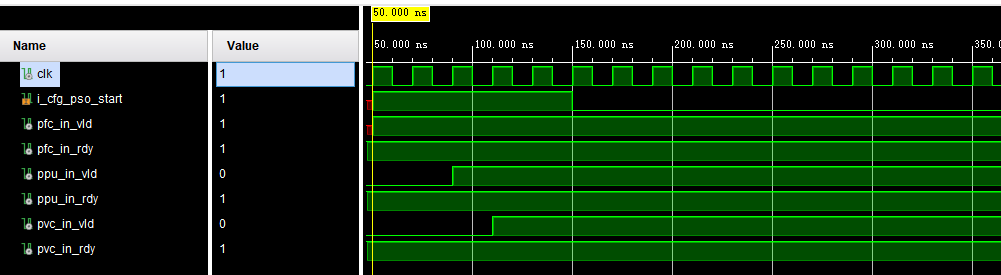
\includegraphics[width=14cm]{fig/5-fig/多起点训练时序图.jpg}
    \caption{多起点训练时序图}
    \label{fig:多起点训练时序图}
\end{figure}

如图\ref{fig:多起点训练时序图}所示,由于是一个6级流水线的设计,所以将训练起点个数设为5就可以完美掩盖流水线的初始延迟,各级模块在开始工作之后,除非因为数据不足、阻塞等原因使得流水线反压导致模块空闲,其余情况下各模块都处于工作状态,硬件利用率较高。需要强调的是,虽然采用多起点训练的方法,但是种群信息更新模块仍然只有一份,所以这5个起点在进行速度和位置更新时使用的是同一份种群最优位置和个体最优位置,所以这并不会对粒子群算法的效果造成太大影响,但这需要在寄存器配置的时候注意一下。

如表\ref{tab:粒子群算法加速补偿系统接口信号表}所示,按照配置顺序,粒子群算法加速补偿系统共有i$\_$cfg$\_$pso$\_$in$\_$initial$\_$para、i$\_$cfg$\_$pso$\_$in$\_$initial$\_$lastv、i$\_$cfg$\_$pso$\_$in$\_$len、i$\_$cfg$\_$pso$\_$start4组寄存器,其中start寄存器只能维持5个周期的高电平,这5个周期内的para寄存器值和lastv寄存器值即为5个训练起点。

\section{双差分验证框架}
由于数字电路不像软件那样出了错误可以随时更改,所以数字电路往往需要经过非常完备的验证以确定其功能的正确性与可靠性。在\ref{RTL model验证框架}节中介绍了硬化后算法与原始补偿算法之间的差分验证环境,通过验证多组虚拟激励和真实数据以保障硬化后算法的正确性,而正确的RTL model在RTL的验证环境中会作为参考的模型,即在原始补偿算法-RTL model、RTL model-RTL之间进行两次差分比较,称为双差分验证框架,其示意图如图\ref{fig:双差分验证环境框架图}所示。三角箭头表示数据类型为数值,菱形箭头表示数据类型为文本,蓝色线条代表进制为十六进制,绿色线条代表进制为二进制,黑色线条代表该处为其他类型操作(比较、控制等),并且在原先4个组成部件:stimulator、RTL model、software、scoreboard的基础上多了一个部分:RTL,RTL为根据RTL model设计出来的门级电路。由于RTL仿真采用的是vivado,而验证环境、原始补偿算法以及参考模型都是使用matlab编写,而vivado和matlab两者之间的兼容性并不算优秀,所以使用verilog自带的系统函数\$fopen和\$fdisplay,将每一个模块级每个计算周期的所有中间结果值写入txt文件,后续验证环境抓取vivado产生的txt文件进行对比分析。需要强调的是,式\eqref{eq:粒子群算法速度更新}中的两个随机数是由两个LSFR产生的,为了保证RTL、RTL model以及原始补偿算法的输入激励一样,需要将LSFR产生的随机数写入txt文件,供验证环境抓取使用,这就导致两次仿真不是同时进行的,必须先在vivado中进行RTL的仿真,生成对应的激励文件之后,才能在matlab中完成后续的仿真以及对比分析。
\begin{figure}[htb]
    \centering
    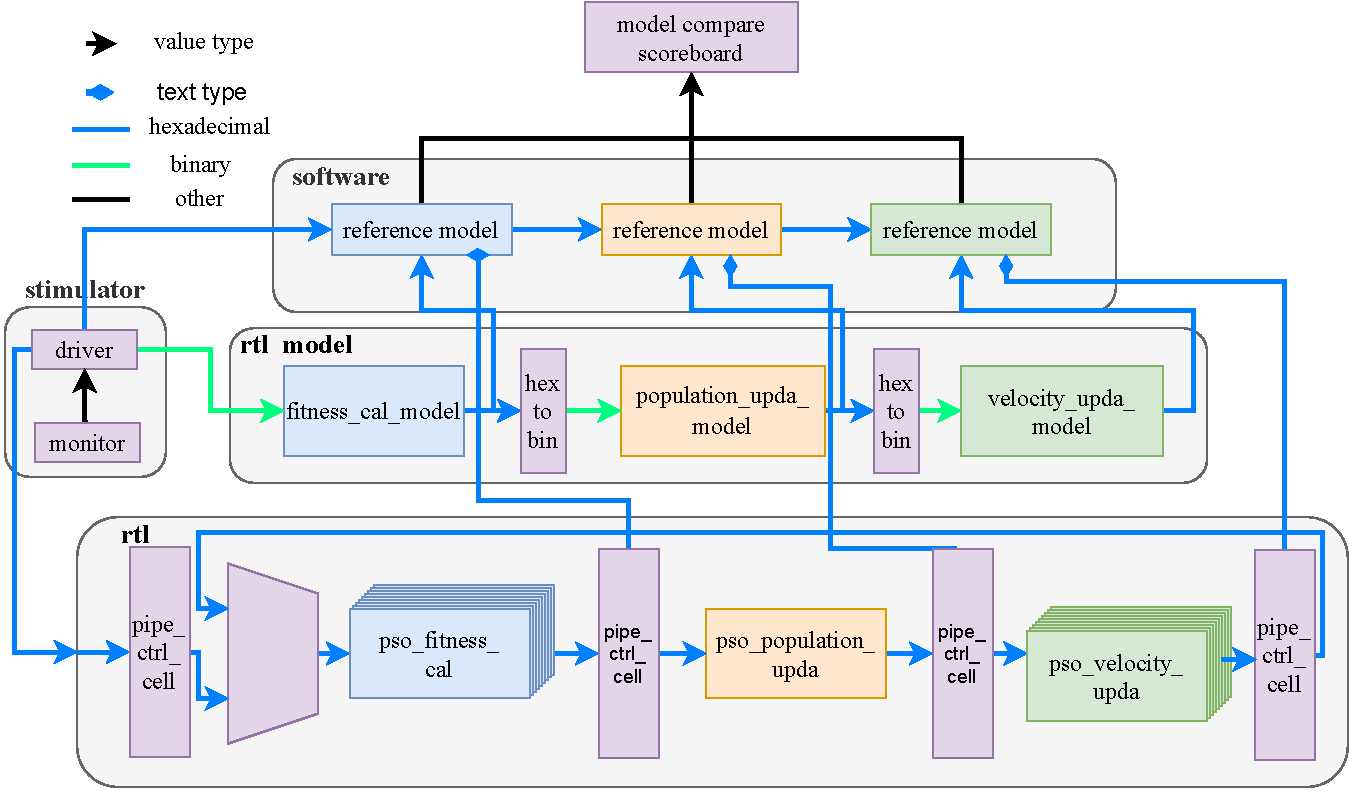
\includegraphics[width=14cm]{fig/5-fig/双差分验证环境.drawio.pdf}
    \caption{双差分验证环境框架图}
    \label{fig:双差分验证环境框架图}
\end{figure}

跟RTL model的验证一样,输入的激励有两种:真实数据和随机产生的虚拟数据,真实数据需要先进行处理,让其变为0.0039的整数倍后才能用于验证,而随机产生的虚拟数据激励如表\ref{tab:RTL激励产生约束}所示。
\begin{table}[H]
    \centering
    \caption{RTL 激励产生约束}
    \label{tab:RTL激励产生约束}
    \begin{tabular}{c|c|c}
        \hline
        激励名                                    & 激励意义                   &  数值范围                  \\ \hline
        pso$\_$fitness$\_$cal$\_$disp            & 输入的位移                  &  [-32768,32767]           \\ \hline
        pso$\_$fitness$\_$cal$\_$pres            & 输入的气压                  &  [-32768,32767]           \\ \hline
        pso$\_$fitness$\_$cal$\_$temp            & 输入的温度                  &  [-32768,32767]           \\ \hline
        pso$\_$population$\_$upda$\_$gbest       & 初始的全局最优解            &  32767                     \\ \hline
        pso$\_$population$\_$upda$\_$pbest       & 初始的局部最优解            &  32767                     \\ \hline
        pso$\_$velocity$\_$upda$\_$para         & 初始的位置信息               & [-500,500]                \\ \hline
        pso$\_$velocity$\_$upda$\_$v            & 初始的速度增量               & [0,1]                      \\ \hline
        pso$\_$velocity$\_$upda$\_$seed         & LSFR的随机种子              & [0,255]                 \\ \hline
    \end{tabular}
  \end{table}

而在进行对比分析时,种群信息更新模块pso$\_$population$\_$upda的输出需要与RTL model的完全一致,而适应度计算模块pso$\_$fitness$\_$cal和速度和位置更新模块pso$\_$velocity$\_$cal的输出允许与RTL model有最大不超过0.0039的误差。随机产生的虚拟数据共生成了20组,每组2500个样本点,共计50000个激励测试点,所有结果的误差都不超过上述设定的条件,并且所以处理后的真实数据也都通过了验证。

\section{本章小结}
本章主要介绍了用于干涉仪环境补偿的粒子群算法加速补偿系统的硬件设计方案,首先从吞吐率这一指标出发,介绍了流水线设计的本质和必要性,随后介绍了粒子群加速补偿系统中的流水线设计方案以及对应的握手控制方案及模块pipe$\_$ctrl$\_$cell的时序图、接口、结构和资源消耗;在通用的设计技术上介绍了逻辑复制与资源共享技术,并介绍了逻辑复制技术在粒子群算法加速补偿系统中种群信息更新模块pso$\_$population$\_$upda中的应用;在功耗设计方面,介绍了基于各模块busy信号的锁存门控时钟方案;在随机数生成设计方面,介绍了基于8位线性反馈移位寄存器的随机数生成方案。然后介绍了整个粒子群算法加速补偿系统的总体硬件架构,以及适应度计算模块、种群信息更新模块和速度和位置更新模块的具体架构,也给出各层级的接口定义。最后介绍了在验证方面提出的基于matlab环境的原始补偿算法-RTL model、RTL model-RTL之间双差分验证框架,也介绍了具体的验证激励和验证结果。
